\documentclass[11pt]{article}

\usepackage[utf8]{inputenc}
\usepackage[T1]{fontenc}
\usepackage[margin=1in]{geometry}
\usepackage{hyperref}
\usepackage{xurl}
\usepackage{url}
\usepackage{booktabs}
\usepackage{amsfonts}
\usepackage{amsmath}
\usepackage{graphicx}
\usepackage{xcolor}
\usepackage{array}
\usepackage{microtype}
\usepackage{placeins}
\usepackage{tikz}
\usetikzlibrary{arrows.meta,positioning,calc,shapes.geometric,fit,backgrounds}

\emergencystretch=1.8em

\hypersetup{
  colorlinks=true,
  linkcolor=blue!60!black,
  urlcolor=blue!60!black,
  citecolor=blue!60!black,
  pdftitle={KAIST IS631 Assignment 3 Report - Virgile Thonnier (20266480)},
  pdfauthor={Virgile Thonnier},
}

\setlength{\parskip}{0.45em}
\setlength{\parindent}{0pt}

\title{\textbf{IS631 Kernel \& System Security: Term Project Assignment 3}\\
\large Implementation and Empirical Evaluation of Authenticated Shared-Memory Latent IPC and Edge Tensor Monitoring in Multi-Agent Systems}

\author{%
  \textbf{Virgile Thonnier} (Student ID: \texttt{20266480})\\
  School of Computing, KAIST\\
  \texttt{virgile.thonnier@kaist.ac.kr}
}

\date{November 27, 2026}

\begin{document}
\maketitle

\section{Executive Summary and Continuity from Assignments 1 \& 2}
In Assignment 1, we initially motivated OS-level sandboxing for emerging AI operating systems (AIOS); in Assignment 2, following the Week~6 seminar on \emph{Out of Sight, Not Out of Mind}~\cite{outofsight}, we focused our system design on a critical blind spot in Latent Multi-Agent Systems (MAS)~\cite{latentmas,c2c}: replacing human-readable inter-agent text messages with direct Key--Value (KV) attention-cache handoffs blinds traditional text message filters and own-activation probes such as AcMAS (Activation-based Multi-Agent Security)~\cite{acmas}. Assignment 2 introduced full-space Projected Gradient Descent (PGD) over outgoing KV tensors (\texttt{M3}--\texttt{M5}) and outlined our Assignment 3 plan to complete multi-suite benchmark validation, investigate zero-shot and black-box boundaries, and package a defensive OS-level runtime. Throughout this report, labels \texttt{M3}--\texttt{M12} identify our modular experiment suites (matching the executable scripts \texttt{run\_m*.py} and verified JSON logs in \texttt{paper/results/}).

In Assignment 3, we unify both threads into a complete user-level Linux prototype and evaluation artifact (\emph{Silent Zombies}) in Python/PyTorch, comprising: (1) a POSIX \texttt{/dev/shm} (Linux RAM-backed \texttt{tmpfs} shared memory) zero-copy inter-process communication (IPC) tensor bus (\texttt{SharedMemoryTensorBus}) protected with keyed HMAC-SHA256 integrity tags; (2) an active edge reference monitor (\texttt{EdgeTensorReferenceMonitor}) combining cryptographic verification with cosine, norm-ratio, and spectral anomaly gating; (3) six adversarial optimization and transfer engines running at inference time without modifying victim model weights; and (4) an end-to-end validation suite spanning $3$ AgentDojo tool-use suites~\cite{agentdojo} ($24$ pairs), $5$ Microsoft TAMAS (\emph{Threats and Attacks in Multi-Agent Systems}) domains~\cite{tamas} ($20$ workflows), LatentMAS~\cite{latentmas} collaborative reasoning on \texttt{GSM8K} (arithmetic word problems) and \texttt{ARC-Challenge} (multiple-choice science questions, $30$ tasks total), multi-hop topology benchmarks, a black-box threat spectrum, and Linux \texttt{/dev/shm} IPC latency measurements. All $14$ unit tests pass locally, and all $10$ primary GPU experiment artifacts (\texttt{M3}, \texttt{M4d}, \texttt{M6}--\texttt{M12}) completed cleanly on Ubuntu 24.04.4 LTS (Linux kernel \texttt{6.6.159+}).

\section{System Implementation and Architecture}
The deliverable codebase under \texttt{latent\_mas\_attack/} implements four coupled subsystems, illustrated topologically in Figure~\ref{fig:ipc_topology}:

\begin{figure}[h]
\centering
\resizebox{\linewidth}{!}{%
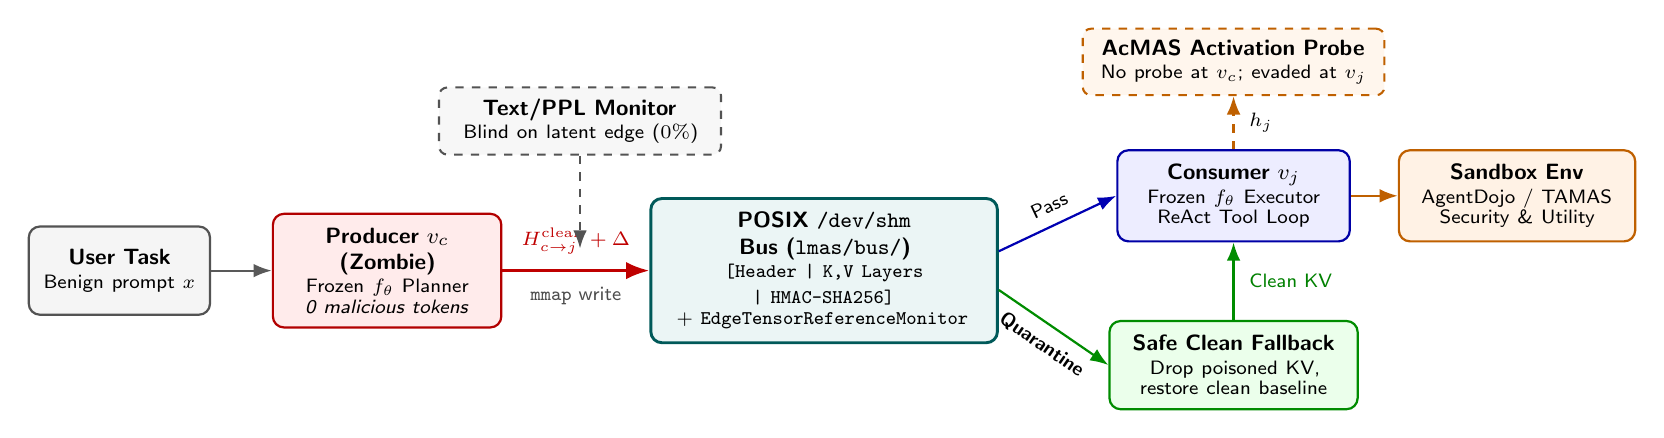
\begin{tikzpicture}[
  >=Latex,
  font=\sffamily\footnotesize,
  nodebox/.style={draw, rounded corners=4pt, align=center, minimum height=1.12cm, inner sep=5pt, line width=0.8pt},
  monbox/.style={draw, rounded corners=3pt, align=center, inner sep=4pt, line width=0.75pt}
]
  \node[nodebox, fill=gray!8, draw=gray!65!black, text width=1.95cm] (user) at (0, 0)
    {\textbf{User Task}\\[-1pt]{\scriptsize Benign prompt $x$}};

  \node[nodebox, fill=red!8, draw=red!70!black, text width=2.55cm] (zombie) at (3.40, 0)
    {\textbf{Producer $v_c$ (Zombie)}\\[-1pt]{\scriptsize Frozen $f_\theta$ Planner}\\[-2pt]{\scriptsize \emph{0 malicious tokens}}};

  \node[nodebox, fill=teal!8, draw=teal!70!black, line width=1.05pt, text width=4.05cm] (bus) at (8.95, 0)
    {\textbf{POSIX \texttt{/dev/shm} Bus (\texttt{lmas/bus/})}\\[-1pt]{\scriptsize \texttt{[Header | K,V Layers | HMAC-SHA256]}}\\[-2pt]{\scriptsize + \texttt{EdgeTensorReferenceMonitor}}};

  \node[nodebox, fill=blue!7, draw=blue!65!black, text width=2.6cm] (exec) at (14.15, 0.95)
    {\textbf{Consumer $v_j$}\\[-1pt]{\scriptsize Frozen $f_\theta$ Executor}\\[-2pt]{\scriptsize ReAct Tool Loop}};

  \node[nodebox, fill=green!8, draw=green!55!black, text width=2.8cm] (safe) at (14.15, -1.20)
    {\textbf{Safe Clean Fallback}\\[-1pt]{\scriptsize Drop poisoned KV,}\\[-2pt]{\scriptsize restore clean baseline}};

  \node[nodebox, fill=orange!10, draw=orange!75!black, text width=2.65cm] (act) at (17.75, 0.95)
    {\textbf{Sandbox Env}\\[-1pt]{\scriptsize AgentDojo / TAMAS}\\[-2pt]{\scriptsize Security \& Utility}};

  \node[monbox, dashed, fill=gray!6, draw=gray!65!black, text width=3.3cm] (txtmon) at (5.85, 1.90)
    {\textbf{Text/PPL Monitor}\\[-1pt]{\scriptsize Blind on latent edge ($0\%$)}};

  \node[monbox, dashed, fill=orange!7, draw=orange!75!black, text width=3.55cm] (acmas) at (14.15, 2.65)
    {\textbf{AcMAS Activation Probe}\\[-1pt]{\scriptsize No probe at $v_c$; evaded at $v_j$}};

  \draw[->, thick, draw=gray!70!black] (user.east) -- (zombie.west);
  \draw[->, very thick, draw=red!75!black] (zombie.east) --
    node[above=2pt, font=\sffamily\scriptsize\bfseries, text=red!75!black] {$H^{\mathrm{clean}}_{c\to j}+\Delta$}
    node[below=2pt, font=\sffamily\scriptsize, text=gray!60!black] {\texttt{mmap} write} (bus.west);

  \draw[->, dashed, thick, draw=gray!65!black] (txtmon.south) -- (5.85, 0.28);
  \draw[->, dashed, thick, draw=orange!75!black] (exec.north) -- node[right=2pt, font=\sffamily\scriptsize] {$h_j$} (acmas.south);

  \draw[->, thick, draw=blue!70!black] ([yshift=7pt]bus.east) --
    node[above=1pt, sloped, font=\sffamily\scriptsize] {Pass} (exec.west);
  \draw[->, thick, draw=green!55!black] ([yshift=-7pt]bus.east) --
    node[below=1pt, sloped, font=\sffamily\scriptsize\bfseries] {Quarantine} (safe.west);
  \draw[->, thick, draw=green!55!black] (safe.north) --
    node[right=2pt, font=\sffamily\scriptsize, text=green!50!black] {Clean KV} (exec.south);
  \draw[->, thick, draw=orange!75!black] (exec.east) -- (act.west);
\end{tikzpicture}}
\caption{Topological architecture of our user-level Linux prototype: \texttt{SharedMemoryTensorBus} and \texttt{EdgeTensorReferenceMonitor} interpose directly on the POSIX \texttt{/dev/shm} latent KV edge $(c\!\to\!j)$ where surface text monitors and post-generation AcMAS probes fail.}
\label{fig:ipc_topology}
\end{figure}

\subsection{POSIX \texttt{/dev/shm} Shared-Memory Tensor Bus (\texttt{lmas/bus/shm\_bus.py})}
In a transformer LLM, processing a prompt of $T$ tokens produces a per-layer \textbf{Key--Value (KV) attention cache} $K^{(\ell)}, V^{(\ell)} \in \mathbb{R}^{1 \times n_{\text{kv}} \times T \times d_h}$ ($n_{\text{kv}}$ KV heads of dimension $d_h$); in a \emph{latent handoff}, an upstream planner transmits this cache directly to a downstream executor, which prepends it to its own attention cache and executes a bounded \textbf{Reason-and-Act (ReAct)} tool loop (iteratively emitting structured JSON tool calls, running them in a sandbox, and reading observations) without decoding natural-language messages. To replace ad-hoc in-memory tensor passing or slow pickle serialization across agent processes, \texttt{SharedMemoryTensorBus} allocates named shared-memory segments under Linux \texttt{/dev/shm} (RAM-backed \texttt{tmpfs} enabling zero-copy \texttt{mmap} IPC). Each edge transfer packs a structured binary header (sequence length, layer count, KV head metadata, dtype tag, sequence nonce) concatenated with raw contiguous layer buffers and a $32$-byte keyed \textbf{HMAC-SHA256} Message Authentication Code computed over the header and tensor payload. If an external writer, bit flip, truncation, or bus spoofing attempt modifies either metadata or tensor bytes in transit, signature verification raises \texttt{BusTamperError} prior to downstream deserialization.

\subsection{Active Edge Tensor Reference Monitor (\texttt{lmas/bus/edge\_monitor.py})}
Text/perplexity (PPL) monitors (\texttt{lmas/detectors/text\_monitor.py}, which combine regex injection patterns with token-perplexity anomaly checks) are blind to continuous KV tensors because no text crosses a latent edge. Likewise, own-activation probes such as \textbf{AcMAS} (\texttt{lmas/detectors/acmas.py}) measure the cosine distance $1-\cos(h_j,\mu_j)$ between a text-generating agent's final hidden state $h_j$ and a benign role centroid $\mu_j$ (flagging above $\tau=0.12$); a non-generating ``silent zombie'' planner emits no text tokens and therefore exposes no generation-time probe point, while downstream states $h_j$ can be regularized back toward $\mu_j$. Furthermore, cryptographic HMAC-SHA256 alone only authenticates transport integrity against external bus tampering---an already-compromised zombie holding its own valid signing key can still sign an adversarially crafted tensor.

To close both gaps, \texttt{EdgeTensorReferenceMonitor} interposes directly on the transmitted KV handoff edge $(c\!\to\!j)$ before downstream ingestion and enforces four checks: (i) valid HMAC-SHA256 authentication; (ii) \emph{position-pooled cosine distance} $1-\cos(\bar H,\mu_{\text{edge}})$ (averaging keys and values across token positions into a length-invariant vector and comparing against a calibrated benign handoff centroid, $\tau_{\cos}=0.01$); (iii) \emph{per-layer Frobenius (L2) norm ratio} $\|H^{(\ell)}\|_F / \mu_{\text{norm}}^{(\ell)}$ against benign reference norms ($\tau_{\text{norm}}=1.08$); and (iv) \emph{spectral concentration shift} $|\sigma_1(H^{(\ell)})/\|H^{(\ell)}\|_F - \mu_{\text{spec}}^{(\ell)}|$ ($\tau_{\text{spec}}=0.05$), measuring how strongly layer energy collapses onto its top singular value $\sigma_1$ to catch low-rank/1D steering directions even when global cosine shift is small. When a handoff is flagged (\texttt{mode="gate"}) or fails authentication, the runtime quarantines the poisoned KV cache and falls back safely to clean unperturbed inference (with an optional per-layer norm-clipping sanitizer \texttt{mode="project"}).

\subsection{Inference-Time, Victim-Unmodified Attack Modules (\texttt{lmas/attacks/} \& \texttt{run\_m*.py})}
Every attack leaves all victim transformer parameters $\theta$, system prompts, and tool definitions completely unmodified at inference time. Our white-box attacks assume access to open victim weights $\theta$ (enabling exact backpropagation gradients $\nabla_\Delta\mathcal{L}$), whereas our black-box attacks use zero victim gradients (\texttt{torch.no\_grad}):
\begin{itemize}
  \item \textbf{Full-Space KV PGD (\texttt{lmas/attacks/pgd.py}, \texttt{run\_m3\_pgd.py}, \texttt{run\_m6\_benchmark.py}):} Optimizes \emph{all coordinates} of both key and value tensors (\texttt{K+V}) across all positions and heads in a target layer subset $\mathcal{S}$ via Adam ($\text{lr}=0.02$), minimizing teacher-forced target tool-call \textbf{Negative Log-Likelihood (NLL)} ($-\sum_t \log p_\theta(s_t\mid s_{<t},\dots)$, where $\text{NLL}\approx 0$ means near-$100\%$ chance of emitting the exact unauthorized JSON call and $\text{NLL}\sim 100$ means near-zero chance). Each step projects perturbed layers onto an L2 norm ball capped by multiplicative ratio $\rho \in \{4, 8, 16\}$ ($\|H^{\text{clean},(\ell)}+\Delta^{(\ell)}\|_2 \le \rho \|H^{\text{clean},(\ell)}\|_2$).
  \item \textbf{White-Box Discrete GCG, 1D Steering, \& Text Conversation Points (\nolinkurl{run_m9_whitebox_matrix_convpoint.py}):} Compares full-space PGD against (a) discrete \textbf{GCG} (Greedy Coordinate Gradient~\cite{zou2023gcg}, iteratively swapping tokens in a $12$-token adversarial text suffix via embedding gradients, over text or encoded into KV), and (b) rank-$1$ \textbf{1D Out-of-Sight (OoS)} steering~\cite{outofsight} (adding a single fixed displacement vector derived from contrasting malicious vs.\ benign prompts). Part~B evaluates \textbf{text conversation points}---inter-agent edges where an agent must decode its latent state into human-readable text tokens that the next agent re-encodes---in a $3$-agent pipeline (\texttt{Planner}$\to$\texttt{Coordinator}$\to$\texttt{Executor}), testing $0$ text boundaries (pure-latent 2-hop PGD) against $1$--$2$ text boundaries (unadapted 1-hop PGD, relay-adapted PGD forcing the Coordinator to verbalize the injection, early text GCG, and all-text).
  \item \textbf{Universal Zero-Shot KV Payloads (\texttt{run\_m10\_transferability.py}):} Standard per-query KV PGD matches one prompt's exact token length $T$ and cannot be added to an unseen prompt of length $T'\neq T$. To achieve \emph{zero-shot} transfer ($0$ test-time gradient steps), we train two length-agnostic payloads offline over $3$ source tasks (\texttt{user\_task\_0..2}, layers $\{20,24,28,32\}$, $\rho=8$): (1) a \textbf{1-Slot Broadcast Delta}, a single learned key/value vector of shape $(1, n_{\text{kv}}, 1, d_h)$ per attacked layer added identically across every token position $1\dots T'$ of any unseen clean handoff ($K_{\text{out}}^{(\ell)} = K_{\text{clean}}^{(\ell)} + \Delta K_{\text{bcast}}^{(\ell)}$); and (2) a \textbf{16-Slot Universal KV Prefix Patch}, a fixed block of $16$ learned \emph{virtual KV token slots} of shape $(1, n_{\text{kv}}, 16, d_h)$ per layer (initialized from a neutral $16$-token base KV cache across all $36$ layers with trainable offsets on layers $\mathcal{S}$). At test time on any unseen prompt of arbitrary length $T'$, the zombie concatenates those $16$ virtual slots onto the clean handoff along the sequence dimension, $K_{\text{out}}^{(\ell)} = [K_{\text{clean}}^{(\ell)} \,\|\, K_{\text{base}}^{(\ell)} + \Delta K_{\text{patch}}^{(\ell)}]$ (length $T'+16$), creating a universal KV prefix consumed directly by the downstream executor across unseen prompts, topologies, and tool schemas.
  \item \textbf{Dual-Evasion Adaptive PGD (\texttt{lmas/attacks/stealth.py}, \texttt{run\_m5\_stealth.py}, \texttt{run\_m8\_shm\_edge\_defense.py}):} Augments the target NLL loss with differentiable penalties pulling downstream hidden states toward the AcMAS centroid ($\lambda_{\text{acmas}}$) and pooled handoffs toward the Edge Monitor centroid ($\lambda_{\text{edge}}$), sweeping a Pareto trade-off frontier to stress-test statistical vs.\ cryptographic defenses.
  \item \textbf{Black-Box \& C2C Bridge Suite (\texttt{lmas/attacks/search.py}, \texttt{run\_m12\_blackbox.py}):} Tests six zero-gradient black-box regimes: \texttt{BB-0} full-space Evolution Strategies (ES, isotropic Gaussian noise over logprob queries), \texttt{BB-1} Singular Value Decomposition (SVD) Subspace Natural Evolution Strategies (NES, searching inside an $r=16$ orthonormal basis of benign-vs.-malicious KV diffs), \texttt{BB-2} decision-only / hard-label search (observing \emph{only decoded text} via a discrete string reward for valid \texttt{<tool\_call>} syntax, tool name, and arguments), and \texttt{BB-3a/b} cross-model \texttt{Qwen2.5-1.5B}$\to$\texttt{3B} surrogate KV patch transfers either unaligned (\texttt{BB-3a}) or mapped through a closed-form linear ridge-regression Cache-to-Cache (C2C)~\cite{c2c} projection matrix fitted on paired benign prompts (\texttt{BB-3b}).
\end{itemize}

\subsection{Multi-Benchmark Harnesses, Evaluation Metrics, and Unit Test Suite}
Graph executors (\texttt{lmas/graph/topology.py}, \texttt{executor.py}) and benchmark drivers (\texttt{run\_m6}, \texttt{run\_m7}, \texttt{run\_m11}) standardize clean vs.\ attacked execution across AgentDojo, TAMAS, and LatentMAS. Across all benchmarks we report: \textbf{Attack Success Rate (ASR)}---the fraction of pairs where the unauthorized tool call or target wrong answer actually executes and passes programmatic post-execution verification (note that AgentDojo names this predicate \texttt{security}, where \texttt{security=true} means the \emph{attack succeeded} and breached the sandbox, while \texttt{security=false} means the environment stayed safe); \textbf{Benign Utility}---the fraction completing the user's original benign request; and detector \textbf{True Positive Rate (TPR)} and \textbf{False Positive Rate (FPR)}---the fractions of attacked and clean handoffs flagged, respectively. Five unit-test modules in \texttt{tests/} ($14$ tests total) verify \texttt{/dev/shm} HMAC integrity, edge monitor calibration and fallback gating, subspace NES scaling, C2C bridge projection math, and metric parsing on CPU without requiring a GPU.

\section{Explicit Implementation and Evaluation Environment}
Per IS631 Assignment 3 guidelines, the exact primary hardware, kernel, and software runtime recorded verbatim in \texttt{paper/results/env\_info.json} is summarized in Table~\ref{tab:env}. Early single-GPU topology/stealth baselines (\texttt{M4}, \texttt{M4b}, \texttt{M4c}, \texttt{M5}) were executed locally on Windows 11 with an NVIDIA RTX 2080 SUPER ($8$~GB VRAM, \texttt{bfloat16} compute). Because the Tesla T4 (\texttt{sm\_75}) lacks hardware Tensor Core \texttt{bfloat16} instructions (triggering slow software emulation), all primary T4 runs automatically select hardware \texttt{float16} compute over 4-bit NormalFloat (NF4) double-quantized \texttt{Qwen2.5-3B-Instruct} weights ($L=36$ layers, grouped-query attention [GQA] with $2$ shared KV heads of dim $128$, and PyTorch Scaled Dot-Product Attention [SDPA]).

\begin{table}[h]
\centering
\caption{Exact Primary Linux Evaluation Environment (\texttt{paper/results/env\_info.json}).}
\label{tab:env}
\resizebox{\linewidth}{!}{%
\begin{tabular}{ll}
\toprule
Component & Verified Specification \\
\midrule
Deployment Model & User-level Python/PyTorch application with POSIX \texttt{/dev/shm} tmpfs IPC \\
Operating System & Ubuntu 24.04.4 LTS (Noble Numbat) \\
Linux Kernel (\texttt{uname -r}) & \texttt{6.6.159+} (\texttt{\#1 SMP Thu Oct 22 03:07:54 UTC 2026 x86\_64}) \\
GPU & NVIDIA Tesla T4 ($14.56$~GB VRAM, compute capability \texttt{sm\_75}) \\
Host Memory & $50$~GiB system RAM \\
Software Stack & Python \texttt{3.13.16}, PyTorch \texttt{2.14.1+cu130}, CUDA \texttt{13.0} \\
ML \& Benchmark Packages & \texttt{transformers 4.53.3}, \texttt{bitsandbytes 0.50.2}, \texttt{agentdojo 0.1.35} \\
Victim Model & \texttt{Qwen/Qwen2.5-3B-Instruct} (4-bit NF4, \texttt{float16} compute, SDPA) \\
\bottomrule
\end{tabular}}
\end{table}

\section{Evaluation Plan and Benchmark Characteristics}
Our evaluation validates both offensive attack efficacy and OS/edge defensive effectiveness across five complementary workloads:
\begin{enumerate}
  \item \textbf{AgentDojo Multi-Suite (\texttt{M3}, \texttt{M6}, \texttt{M7}, \texttt{M9}):} $24$ user/injection pairs ($8$ each across \texttt{workspace} email/calendar/files, \texttt{banking} transfers, and \texttt{slack} messaging) measuring programmatic post-execution unauthorized tool ASR and benign task utility against clean runs, inter-agent text injections, indirect tool injections, white-box discrete GCG, 1D Out-of-Sight steering, and $3$-agent text conversation boundaries.
  \item \textbf{Microsoft TAMAS 4-Agent MAS (\texttt{M11}):} $20$ workflows across $5$ high-stakes domains (\texttt{finance}, \texttt{healthcare}, \texttt{legal}, \texttt{education}, \texttt{news}; $4$ scenarios per domain), comparing clean execution, TAMAS text Direct Prompt Injection (DPI---explicit malicious text appended to queries), Silent Zombie latent PGD, and active edge gating. (Note: the $3$B model already triggers sensitive tools unprompted on $20.0\%$ of clean TAMAS workflows, mostly in \texttt{news}/\texttt{healthcare}, establishing the clean baseline floor.)
  \item \textbf{LatentMAS Reasoning (\texttt{M11}):} $15$ \texttt{GSM8K} (grade-school math word problems) and $15$ \texttt{ARC-Challenge} (multiple-choice science questions) executed by a $4$-agent latent reasoning team (\texttt{Planner}$\to$\texttt{Critic}$\to$\texttt{Refiner}$\to$\texttt{Judger}), quantifying token savings, clean accuracy, exact-target wrong-answer hijack ASR, and edge-monitor recovery.
  \item \textbf{Topology Reach, Zero-Shot Transfer, and Black-Box Boundary (\texttt{M4}--\texttt{M4d}, \texttt{M10}, \texttt{M12}):} Multi-hop \emph{reach} (forced survival of a benign sentinel word \texttt{"BANANA"} across hops in text-mediated depth-$5$ chains vs.\ pure-latent differentiable depths $2$--$6$, plus reconvergent diamond DAGs where two parallel branches merge), $16$-task / $6$-topology / $6$-schema zero-shot transfer, and $6$ zero-gradient black-box attack regimes (\texttt{BB-0} through \texttt{BB-3b}).
  \item \textbf{Linux \texttt{/dev/shm} IPC Microbenchmark (\texttt{M8}):} Synthetic $36$-layer \texttt{bf16} KV caches across sequence lengths $\{64, 256, 512, 1024\}$ ($2.25\text{--}36.00$~MB, $25$ trials per length) comparing authenticated POSIX \texttt{/dev/shm} against unauthenticated \texttt{torch.save} serialization plus $10$ integrity tamper injection tests.
\end{enumerate}

\section{Empirical Results and Analysis}
All results below match the verified JSON files under \texttt{paper/results/} verbatim. Note carefully that in \texttt{M10}, cross-precision evaluation (\texttt{cross\_precision\_bf16}) was skipped in the final Colab sweep to prioritize finishing \texttt{M12}; only the three completed transfer axes are reported, and cross-precision transfer is documented as future work.

\subsection{Latent Action Forcing, White-Box Expressivity, and Text Firewalls (\texttt{M3}, \texttt{M6}, \texttt{M7}, \texttt{M9})}
In \texttt{M3} (Figure~\ref{fig:m3_report}), all four layer/norm configs ($4$ late layers \texttt{late4\_n8}, $4$ spread layers \texttt{spread4\_n8} and \texttt{spread4\_n16}, and $6$ deep layers \texttt{deep6\_n16}, with $\rho\in\{8,16\}$) reduce target \texttt{send\_email} NLL from $\sim 118.4$ below $0.01$ within $\sim 40$ steps ($0.005$--$0.009$ at step $120$) and trigger verified unauthorized email execution (AgentDojo \texttt{security=true}). Scaled to $24$ pairs across $3$ AgentDojo suites (Table~\ref{tab:summary_metrics}), latent PGD achieves $75.0\%$ ASR vs.\ $4.2\%$ for inter-agent and indirect tool text baselines ($100.0\%$ and $83.3\%$ text-monitor catch), while completely evading text and AcMAS detectors ($0.0\%$ catch). Edge gating achieves $50.0\%$ TPR on \texttt{workspace} ($75.0\% \to 25.0\%$ ASR at $0.0\%$ FPR; $16.7\%$ overall TPR).

\begin{figure}[h]
\centering
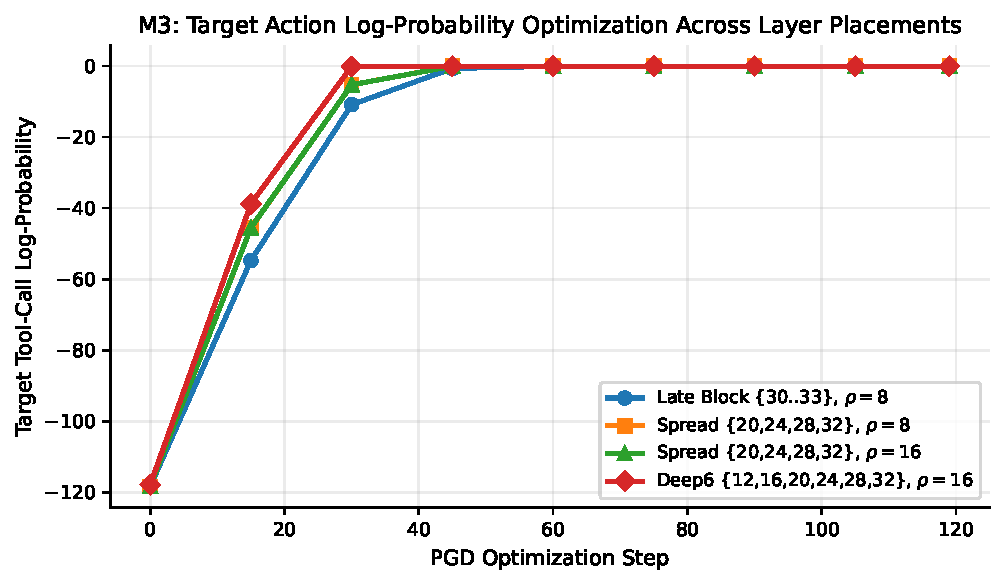
\includegraphics[width=0.68\linewidth]{../paper/figures/fig2_m3_nll_convergence.pdf}
\caption{M3 optimization trajectories across all four PGD layer placements and norm budgets.}
\label{fig:m3_report}
\end{figure}

In the controlled \texttt{M9} white-box matrix (Figure~\ref{fig:m9_report}, $n=8$), full-space KV PGD reaches $62.5\%$ ASR (NLL $0.029$, $64.74$~s), outperforming discrete text WB-GCG ($37.5\%$ ASR, $116.39$~s, $75.0\%$ caught by text/perplexity [PPL] checks), latent WB-GCG ($0.0\%$), and 1D Out-of-Sight steering ($0.0\%$ ASR, NLL $699.344$, $100.0\%$ flagged). Crucially, Part~B reveals that inserting even a single text conversation boundary (forcing an intermediate agent to decode to readable text and re-encode) in a $3$-agent pipeline drops ASR from $62.5\%$ to $0.0\%$ across all four variants while enabling $25.0\%$--$75.0\%$ text monitor detection.

\begin{figure}[h]
\centering
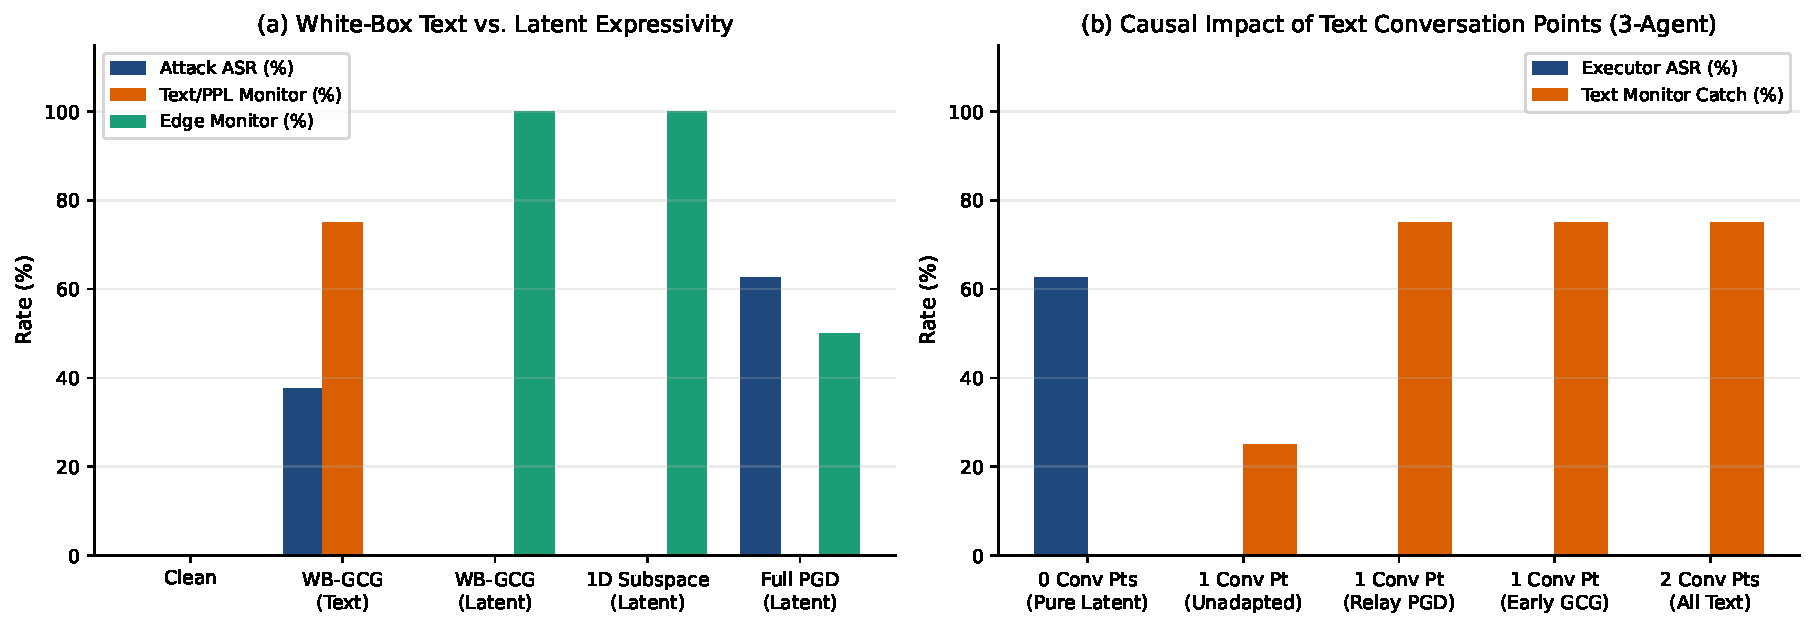
\includegraphics[width=\linewidth]{../paper/figures/fig1_whitebox_matrix_convpoint.pdf}
\caption{M9 white-box expressivity comparison (a) and causal mitigation via text conversation points (b).}
\label{fig:m9_report}
\end{figure}

\subsection{Pure-Latent Unbounded Reach and Zero-Shot Prefix Patch Transfer (\texttt{M4d}, \texttt{M10})}
Figure~\ref{fig:report_topologies} summarizes how graph topology governs latent propagation. Measuring forced survival of the sentinel word \texttt{"BANANA"} across hops, intermediate text decoding caps text-mediated chain reach at $33.3\%$ beyond hop~$2$, whereas removing intermediate decodes in a pure-latent differentiable chain (\texttt{M4d}, Figure~\ref{fig:m5_report}(a)) achieves $100.0\%$ target control across all tested depths $2, 3, 4, 5, 6$ ($n=3$, $\rho=8$) with non-vanishing initial gradient norms ($2.45\text{--}3.23$). Furthermore, \texttt{M10} (Figure~\ref{fig:m10_report}) demonstrates that our length-agnostic $16$-slot Universal KV Prefix Patch (concatenated onto any clean handoff as $[K_{\text{clean}} \| K_{\text{patch}}]$ after offline training on $3$ tasks) transfers zero-shot ($0$ test-time gradient steps) at $81.2\%$ ASR on $16$ unseen tasks ($56.2\%$ for the $1$-slot Broadcast Delta), $50.0\%$ on $3$-worker Star and $3$-hop pure-latent topologies ($n=6$), $33.3\%$ on a single-patch reconvergent DAG ($[H_{\text{patch}} \| H_{\text{clean}}]$, vs.\ $0.0\%$ if naively duplicated on both merged branches), and $50.0\%$ under paraphrased executor prompts and reversed tool schemas.

\begin{figure}[h]
\centering
\resizebox{\linewidth}{!}{%
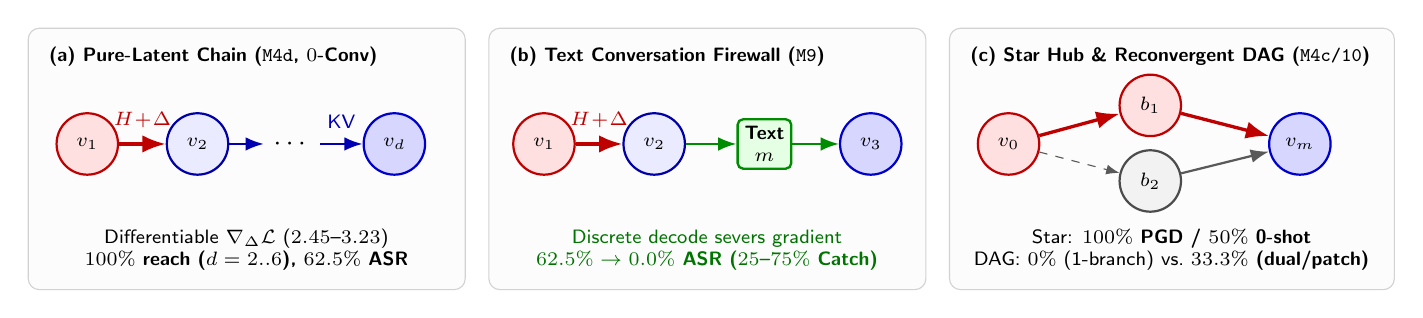
\begin{tikzpicture}[
  >=Latex,
  font=\sffamily\scriptsize,
  ag/.style={circle, draw, minimum size=0.78cm, inner sep=1pt, font=\sffamily\scriptsize\bfseries, line width=0.8pt},
  zom/.style={ag, fill=red!12, draw=red!75!black},
  lat/.style={ag, fill=blue!8, draw=blue!65!black},
  tgt/.style={ag, fill=blue!16, draw=blue!80!black},
  cln/.style={ag, fill=gray!10, draw=gray!60!black},
  panel/.style={draw=gray!35, rounded corners=4pt, fill=gray!2}
]
  % (a) Pure-Latent Chain
  \draw[panel] (0, 0) rectangle (5.55, 3.32);
  \node[anchor=north west, font=\sffamily\scriptsize\bfseries] at (0.14, 3.20)
    {(a) Pure-Latent Chain (\texttt{M4d}, $0$-Conv)};
  \node[zom] (a1) at (0.75, 1.85) {$v_1$};
  \node[lat] (a2) at (2.15, 1.85) {$v_2$};
  \node[font=\sffamily\bfseries] (adots) at (3.35, 1.85) {$\cdots$};
  \node[tgt] (ad) at (4.65, 1.85) {$v_d$};
  \draw[->, very thick, red!75!black] (a1) -- node[above=2pt] {$H\!+\!\Delta$} (a2);
  \draw[->, thick, blue!70!black] (a2) -- (adots);
  \draw[->, thick, blue!70!black] (adots) -- node[above=2pt] {KV} (ad);
  \node[anchor=south, align=center] at (2.77, 0.12)
    {Differentiable $\nabla_\Delta\mathcal{L}$ ($2.45$--$3.23$)\\\textbf{$100\%$ reach ($d=2..6$), $62.5\%$ ASR}};

  % (b) Text Conversation Firewall
  \draw[panel] (5.85, 0) rectangle (11.40, 3.32);
  \node[anchor=north west, font=\sffamily\scriptsize\bfseries] at (5.99, 3.20)
    {(b) Text Conversation Firewall (\texttt{M9})};
  \node[zom] (b1) at (6.55, 1.85) {$v_1$};
  \node[lat] (b2) at (7.95, 1.85) {$v_2$};
  \node[draw=green!55!black, fill=green!10, rounded corners=2pt, inner sep=2.5pt, align=center, line width=0.85pt] (fw) at (9.35, 1.85)
    {\textbf{Text}\\$m$};
  \node[tgt] (b3) at (10.70, 1.85) {$v_3$};
  \draw[->, very thick, red!75!black] (b1) -- node[above=2pt] {$H\!+\!\Delta$} (b2);
  \draw[->, thick, green!55!black] (b2) -- (fw);
  \draw[->, thick, green!55!black] (fw) -- (b3);
  \node[anchor=south, align=center, text=green!45!black] at (8.62, 0.12)
    {Discrete decode severs gradient\\\textbf{$62.5\%\to 0.0\%$ ASR ($25$--$75\%$ Catch)}};

  % (c) Star & Reconvergent DAG
  \draw[panel] (11.70, 0) rectangle (17.35, 3.32);
  \node[anchor=north west, font=\sffamily\scriptsize\bfseries] at (11.84, 3.20)
    {(c) Star Hub \& Reconvergent DAG (\texttt{M4c/10})};
  \node[zom] (d0) at (12.45, 1.85) {$v_0$};
  \node[zom] (db1) at (14.25, 2.34) {$b_1$};
  \node[cln] (db2) at (14.25, 1.38) {$b_2$};
  \node[tgt] (dm) at (16.15, 1.85) {$v_m$};
  \draw[->, very thick, red!75!black] (d0) -- (db1);
  \draw[->, dashed, gray!70!black] (d0) -- (db2);
  \draw[->, very thick, red!75!black] (db1) -- (dm);
  \draw[->, thick, gray!70!black] (db2) -- (dm);
  \node[anchor=south, align=center] at (14.52, 0.12)
    {Star: \textbf{$100\%$ PGD / $50\%$ 0-shot}\\DAG: $0\%$ (1-branch) vs.\ \textbf{$33.3\%$ (dual/patch)}};
\end{tikzpicture}}
\caption{Evaluated multi-agent communication topologies: (a) pure-latent chains propagate perturbations losslessly across $6$ hops; (b) a single text boundary acts as a causal security firewall; and (c) star hubs fan out while reconvergent DAGs dilute single-branch cascades.}
\label{fig:report_topologies}
\end{figure}

\begin{figure}[h]
\centering
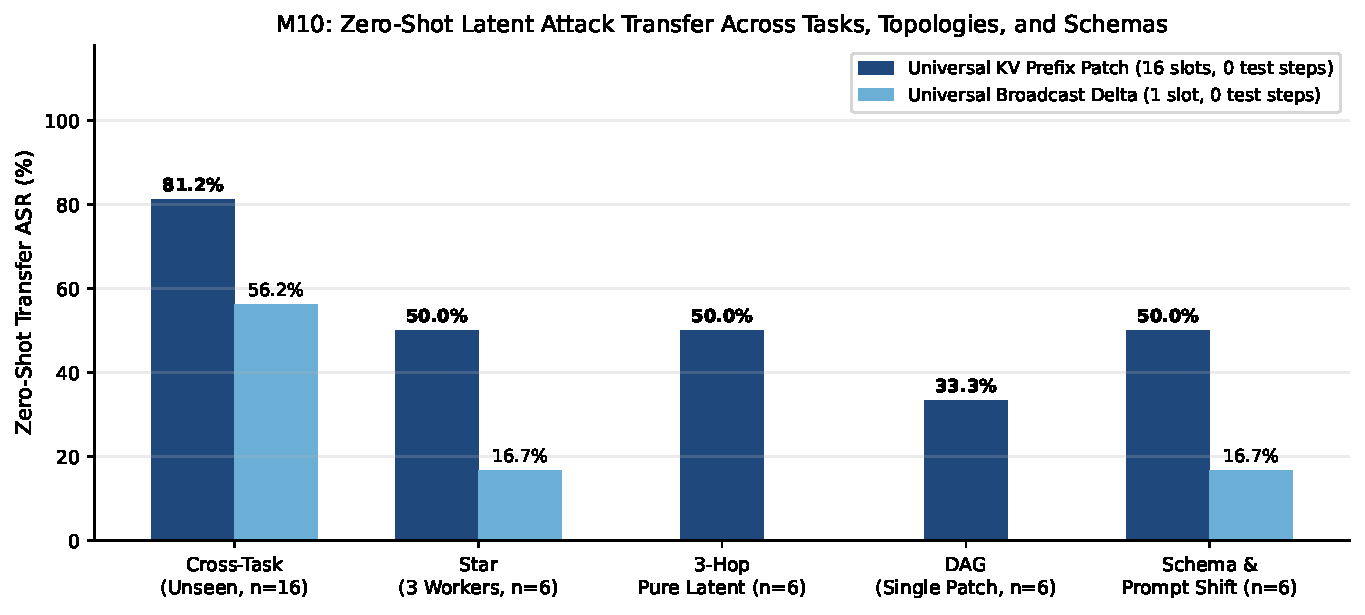
\includegraphics[width=0.84\linewidth]{../paper/figures/fig3_transferability.pdf}
\caption{M10 zero-shot transferability with zero test-time optimization steps across tasks, topologies, and schemas.}
\label{fig:m10_report}
\end{figure}

\subsection{TAMAS, LatentMAS, Adaptive Stealth, and Linux \texttt{/dev/shm} IPC Performance (\texttt{M8}, \texttt{M11})}
Table~\ref{tab:summary_metrics} and Figure~\ref{fig:m11_report} show \texttt{M11} outcomes on Microsoft TAMAS and LatentMAS. On TAMAS ($20$ workflows), Silent Zombie PGD hits $100.0\%$ ASR across all $5$ domains with $0.0\%$ text catch and $45.0\%$ AcMAS catch ($0.0\%$ on \texttt{education}/\texttt{news}), whereas \texttt{EdgeTensorReferenceMonitor} catches $100.0\%$ of attacks and restores exact clean baseline security ($20.0\%$ ASR) and utility ($65.0\%$). On LatentMAS, KV handoffs cut tokens by $94.7\%$ (\texttt{GSM8K}: $339.8 \to 18.1$ tok/q) and $98.5\%$ (\texttt{ARC-Challenge}: $205.7 \to 3.0$ tok/q); full-space PGD hijacks $53.3\%$ (\texttt{GSM8K}) and $100.0\%$ (\texttt{ARC}) of answers vs.\ $0.0\%$ for 1D Out-of-Sight, while Edge gating achieves $100.0\%$ TPR and restores clean latent accuracy ($13.3\%$ and $60.0\%$).

\begin{figure}[h]
\centering
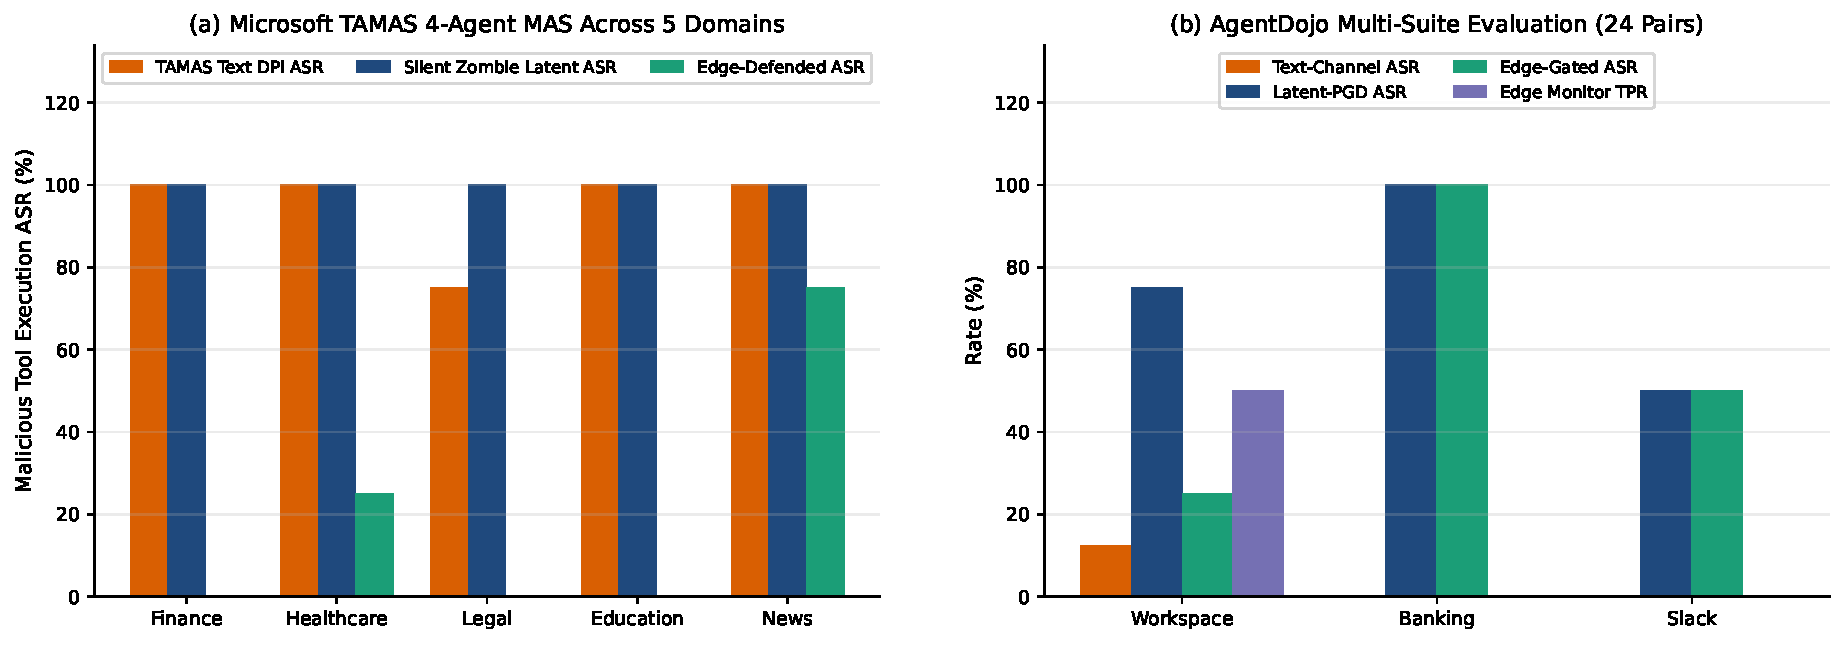
\includegraphics[width=\linewidth]{../paper/figures/fig4_mas_benchmarks.pdf}
\caption{M11 Microsoft TAMAS 5-domain protection (a) and M6/M7 AgentDojo 24-pair comparison (b).}
\label{fig:m11_report}
\end{figure}

In \texttt{M8} dual-evasion (Figure~\ref{fig:m5_report}(b)), setting $\lambda_{\text{acmas}}=20$ alone leaves $66.7\%$ caught by Edge Monitor; adding $\lambda_{\text{edge}}=2500$ compresses edge cosine distance $10.8\times$ ($0.01112 \to 0.00103$, norm ratio $1.0514 \to 1.0094$), bypassing unauthenticated statistical thresholds ($0.0\%$ flag rate at $100.0\%$ ASR). On Linux kernel \texttt{6.6.159+} \texttt{/dev/shm} (Figure~\ref{fig:m8_report}), HMAC-SHA256 authentication rejects $10/10$ tampered segments ($100.0\%$) against external bus spoofing or corruption. Crucially, software HMAC-SHA256 throughput ($0.134\text{--}0.152$~GB/s) dominates copy latency ($16.41\text{--}236.07$~ms vs.\ $11.20\text{--}64.41$~ms for unauthenticated serialization across $2.25\text{--}36.00$~MB payloads), pointing directly to hardware-accelerated Authenticated Encryption with Associated Data (AEAD) or Network Interface Card (NIC) / Compute Express Link (CXL) offload as a kernel systems optimization.

\begin{figure}[h]
\centering
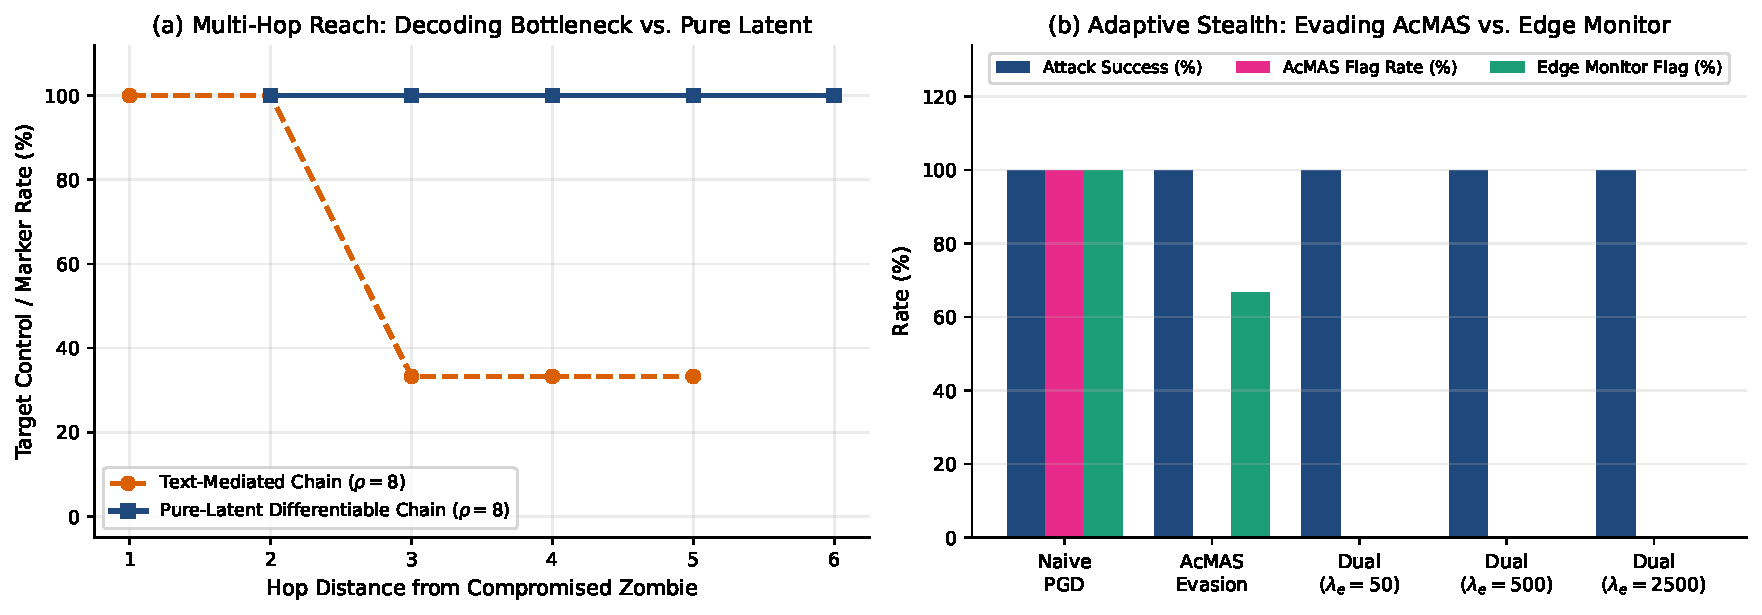
\includegraphics[width=\linewidth]{../paper/figures/fig5_reach_and_stealth.pdf}
\caption{Multi-hop reach (a) and adaptive dual-evasion Pareto behavior (b).}
\label{fig:m5_report}
\end{figure}

\begin{figure}[h]
\centering
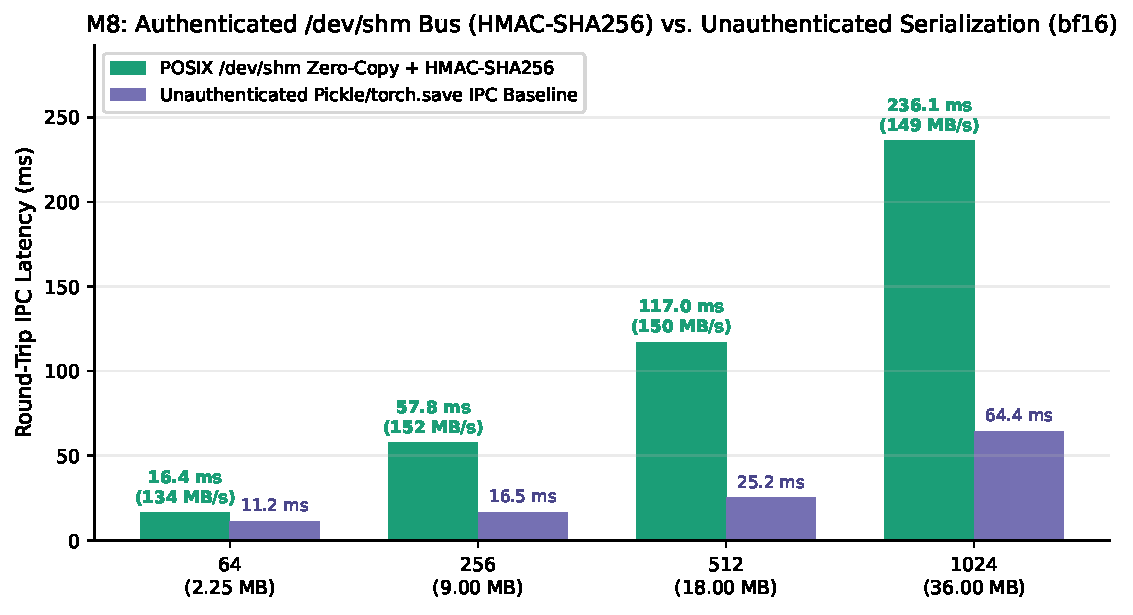
\includegraphics[width=0.72\linewidth]{../paper/figures/fig6_shm_bus_latency.pdf}
\caption{M8 Linux \texttt{/dev/shm} zero-copy + HMAC-SHA256 IPC latency vs.\ unauthenticated serialized baseline.}
\label{fig:m8_report}
\end{figure}

\subsection{Black-Box Threat Boundary (\texttt{M12})}
Every zero-gradient black-box regime in \texttt{M12} (\texttt{BB-0} full-space ES $60$q, \texttt{BB-1} SVD subspace NES $241$q, \texttt{BB-2} decision-only $25$q---which achieves partial \texttt{<tool\_call>} tag syntax on $3/6$ pairs for mean string reward $0.50$ but fails semantic arguments---, \texttt{BB-3a} unaligned \texttt{1.5B}$\to$\texttt{3B} surrogate transfer, and \texttt{BB-3b} C2C linear ridge-regression bridges) scores $0.0\%$ unauthorized tool-call ASR across $6$ pairs (mean NLL $91.84\text{--}147.16$; \texttt{BB-1}/\texttt{BB-2} $100.0\%$ caught by Edge Monitor), vs.\ $62.5\%$ ASR (NLL $0.029$) for white-box PGD (Figure~\ref{fig:m12_report}). Protecting weights and KV internal layouts thus establishes a strong perimeter against external query-only attackers.

\begin{figure}[h]
\centering
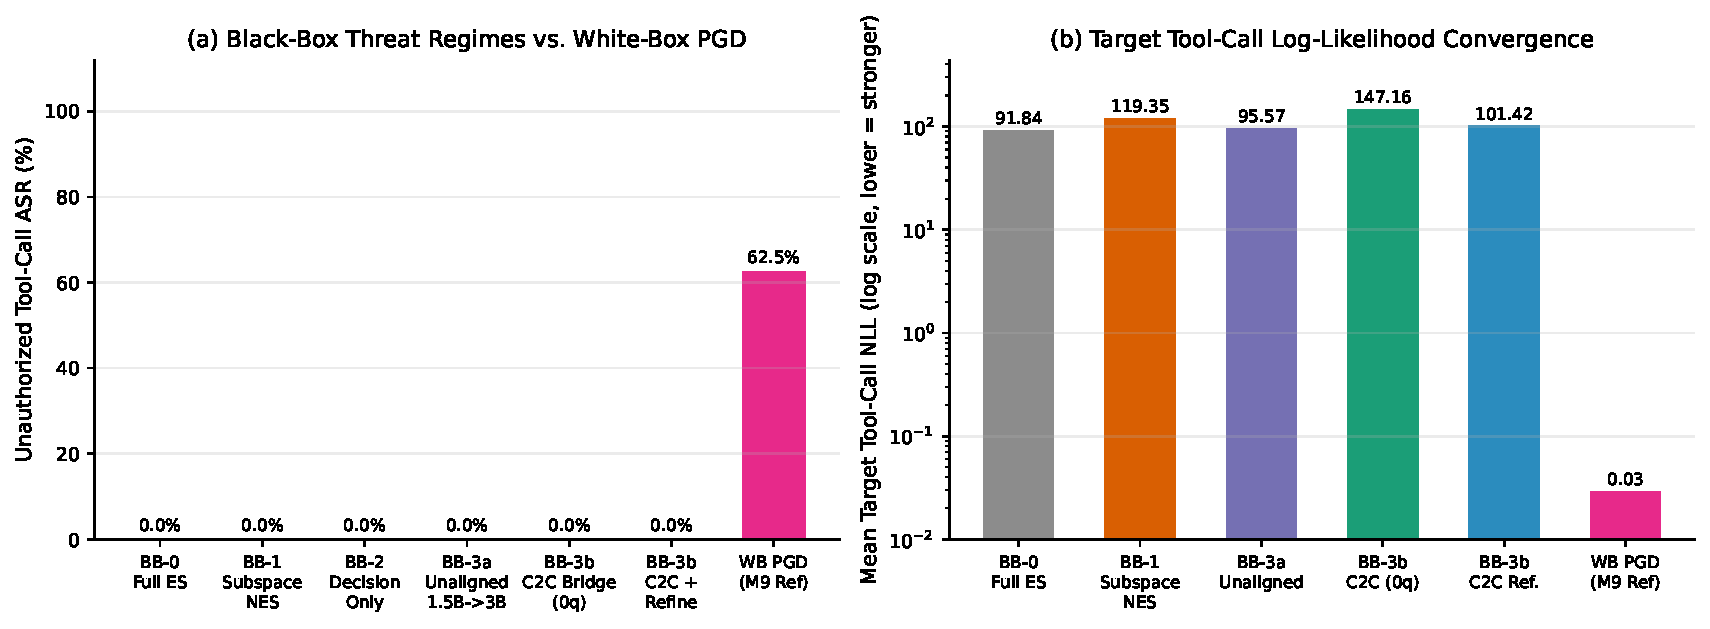
\includegraphics[width=\linewidth]{../paper/figures/fig7_blackbox.pdf}
\caption{M12 black-box regimes vs.\ white-box PGD: ASR (a) and mean target tool-call NLL (b).}
\label{fig:m12_report}
\end{figure}

\begin{table}[h]
\centering
\caption{Consolidated Verified Headline Results Across Benchmarks (\texttt{paper/results/*.json}).}
\label{tab:summary_metrics}
\resizebox{\linewidth}{!}{%
\begin{tabular}{llccc}
\toprule
Experiment & Condition & Primary Metric (ASR / Acc) & Text Catch & AcMAS / Edge Catch \\
\midrule
\texttt{M6}/\texttt{M7} AgentDojo ($n=24$) & Clean / Text / Latent PGD & $0.0\%$ / $4.2\%$ / $\mathbf{75.0\%}$ & --- / $100\%$ / $0\%$ & $0\%$ / $16.7\%$ ($50\%$ ws) \\
\texttt{M9} Matrix ($n=8$) & WB-GCG (Text) / Full PGD (Latent) & $37.5\%$ / $\mathbf{62.5\%}$ & $75.0\%$ / $0.0\%$ & $0\%$ / $50.0\%$ \\
\texttt{M9} Conv.\ Pts ($n=8$) & $0$ Text Pts / $\ge 1$ Text Pt & $62.5\%$ / $\mathbf{0.0\%}$ & $0.0\%$ / $25$--$75\%$ & --- \\
\texttt{M10} Transfer & Unseen Task ($n=16$, 16-slot Patch) & $\mathbf{81.2\%}$ zero-shot & --- & --- \\
\texttt{M11} TAMAS ($n=20$) & Clean / Text DPI / Latent / Edge Def. & $20\%$ / $95\%$ / $100\%$ / $\mathbf{20\%}$ & --- / $100\%$ / $0\%$ / --- & $45\%$ / $\mathbf{100.0\%}$ \\
\texttt{M11} LatentMAS \texttt{GSM8K} & Full PGD Hijack / Edge Defended & $53.3\%$ / $\mathbf{0.0\%}$ ($13.3\%$ acc) & --- & --- / $\mathbf{100.0\%}$ \\
\texttt{M11} LatentMAS \texttt{ARC} & Full PGD Hijack / Edge Defended & $100.0\%$ / $\mathbf{20.0\%}$ ($60.0\%$ acc) & --- & --- / $\mathbf{100.0\%}$ \\
\texttt{M12} Black-Box ($n=6$) & \texttt{BB-0}..\texttt{BB-3b} vs.\ \texttt{M9} WB PGD & $\mathbf{0.0\%}$ vs.\ $62.5\%$ & --- & \texttt{BB-1/2}: $100.0\%$ Edge \\
\bottomrule
\end{tabular}}
\end{table}

\FloatBarrier
\section{Reproducibility and Artifact Guide}
All code, tests, raw JSON metrics, PDFs, and Colab drivers are archived inside \texttt{artifact/} of the submission archive and hosted publicly on GitHub and Hugging Face:
\begin{itemize}
  \item \textbf{GitHub Repository:} \url{https://github.com/vthonnier/is631-silent-zombies}
  \item \textbf{Hugging Face Dataset:} \url{https://huggingface.co/datasets/vthonnier/is631-silent-zombies-artifacts}
  \item \textbf{Unit Tests (CPU):} \texttt{python -m pytest -v} ($14/14$ tests pass locally).
  \item \textbf{Figure Regeneration:} \texttt{python scripts/generate\_figures.py} produces \texttt{fig1}--\texttt{fig7} from \texttt{paper/results/*.json}.
  \item \textbf{GPU Sweep:} Execute the notebook \texttt{notebooks/IS631\_Assignment3\_Colab.ipynb}, or invoke the resumable CLI runner \texttt{python scripts/run\_colab\_suite.py}.
\end{itemize}

\section{Generative AI Usage Disclosure (Models \& Documented Prompts)}
In strict accordance with KAIST IS631 submission policy (requiring explicit disclosure of both AI models and concrete prompts for reproducibility), generative AI assistants were used during implementation, remote GPU orchestration, visualization, and LaTeX editing:
\begin{itemize}
  \item \textbf{Models \& Environments:} (1) \textbf{Anthropic Claude Code (\texttt{Claude Opus 5.5})} for initial \texttt{M3}--\texttt{M6} PyTorch attack/topology drivers (as disclosed in Assignment~2); and (2) \textbf{Google Antigravity IDE (\texttt{Google DeepMind Gemini} models)} with the Colab API MCP server for \texttt{/dev/shm} IPC bus \& \texttt{EdgeTensorReferenceMonitor} implementation, \texttt{M7}--\texttt{M12} drivers, headless Tesla~T4 execution, TikZ/matplotlib figures, and report compilation.
  \item \textbf{Documented Prompts (Verbatim / Representative):}
  \begin{enumerate}
    \item \emph{OS Shared-Memory Bus \& Edge Monitor (\texttt{Gemini} in Antigravity):} ``Implement a POSIX \texttt{/dev/shm} zero-copy tensor bus (\texttt{SharedMemoryTensorBus}) with HMAC-SHA256 integrity authentication and an active \texttt{EdgeTensorReferenceMonitor} gating KV handoffs by cosine distance, per-layer norm ratio, and spectral energy, plus CPU unit tests and an \texttt{M8} dual-evasion + IPC latency benchmark.''
    \item \emph{Extended Benchmarks \& Threat Boundary (\texttt{Gemini} in Antigravity):} ``Implement \texttt{M9} (white-box discrete GCG vs.\ 1D Out-of-Sight vs.\ full-space KV PGD and 3-agent text conversation points), \texttt{M10} (zero-shot 1-slot broadcast and 16-slot universal KV prefix patches), \texttt{M11} (Microsoft TAMAS 5 domains and LatentMAS \texttt{GSM8K}/\texttt{ARC-Challenge}), and \texttt{M12} (black-box ES, SVD subspace NES, decision-only search, and \texttt{1.5B}$\to$\texttt{3B} C2C ridge bridges), and run them resumably on Colab T4.''
    \item \emph{Report, Topological Diagrams, \& Submission Audit (\texttt{Gemini} in Antigravity):} ``Add clean LaTeX topological graphs in the paper and Assignment 3 report to explain key mechanisms, verify full IS631 schedule/submission compliance, and generate an animated visual overview for the GitHub repository.''
  \end{enumerate}
  \item \textbf{Human Author Verification:} The author independently verified every scientific claim, inspected all raw JSON artifacts in \texttt{paper/results/} verbatim, ran all $14$ unit tests, visually audited every figure and compiled PDF page, deferred unexecuted sweeps (\texttt{cross\_precision\_bf16}) to future work rather than extrapolating, and reported exact software HMAC-SHA256 overhead ($134\text{--}152$~MB/s) faithfully.
\end{itemize}

\begin{thebibliography}{9}
\footnotesize
\bibitem{latentmas} J.~Zou et al., ``Latent Collaboration in Multi-Agent Systems,'' \emph{ICML}, 2026 (arXiv:2511.20639).
\bibitem{c2c} T.~Fu et al., ``Cache-to-Cache: Direct Semantic Communication Between Large Language Models,'' \emph{ICLR}, 2026 (arXiv:2510.03215).
\bibitem{outofsight} C.~Wang et al., ``Out of Sight, Not Out of Mind: Unveiling Latent Attack in Latent-based Multi-Agent Systems,'' \emph{EMNLP}, 2026 (arXiv:2605.28214).
\bibitem{acmas} H.~Xu et al., ``When Agents Go Rogue: Activation-Based Detection of Malicious Behaviors in Multi-Agent Systems,'' \emph{ICML}, 2026 (arXiv:2607.06807).
\bibitem{agentdojo} E.~Debenedetti et al., ``AgentDojo: A Dynamic Environment to Evaluate Prompt Injection Attacks and Defenses for LLM Agents,'' \emph{NeurIPS Datasets \& Benchmarks}, 2024 (arXiv:2406.13352).
\bibitem{tamas} I.~Kavathekar et al., ``TAMAS: Benchmarking Adversarial Risks in Multi-Agent LLM Systems,'' arXiv:2511.05269, 2025.
\bibitem{zou2023gcg} A.~Zou et al., ``Universal and Transferable Adversarial Attacks on Aligned Language Models,'' arXiv:2307.15043, 2023.
\end{thebibliography}

\end{document}
